\section{Findings}
It has been found that the population and dynamics of an online space
may affect individual user behaviour. Jones, Ravid, Rafaeli find that
Newsgroups users publish shorter posts in more populous threads.  

An interesting case is that of the english Wikipedia page on biologist
Rupert Sheldrake. Rupert Sheldrake is a biologist, who, with his
`astonishingly visionary' early work in plant science had him
described as `one of the brightest Darwinians of his
generation',\cite{odyssey-auxin}\cite{guardianshel}, came under heavy
criticism for his later work in psychical research, and `mysterious
telepathy-type interconnections between organisms and collective
memories within species'.\cite{sheldrake-biog} 

The Wikipedia article history is accordingly erratic, a continuation a
a long history of Sheldrake-bashing, as can be seen in the plots of
figure~\ref{fig:sheldrake-plots}.

\begin{figure}
  \label{fig:sheldrake-plots}
  \centering
  \makebox[\linewidth][c]{
    \begin{subfigure}[b!]{0.6\linewidth}
      \centering
      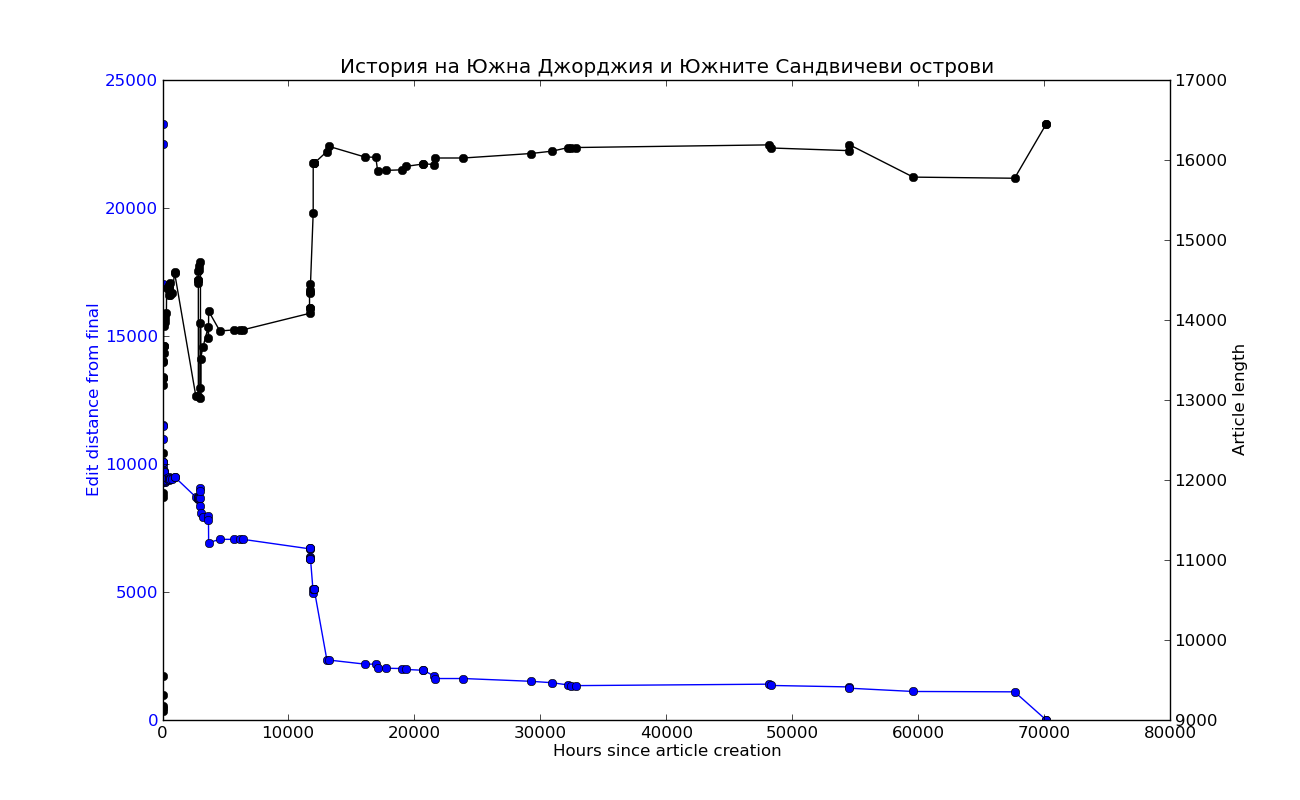
\includegraphics[width=\linewidth]{img/traj-classic/bg90882traj.png}
      \caption{\href{http://bg.wikipedia.org/wiki/index.php?curid=90882}{Bulgarian
      Wikipedia, Page ID 90882 (History of South Georgia and the South Sandwich Islands)}}
    \end{subfigure}
    \begin{subfigure}[b!]{0.6\linewidth}
      \centering
      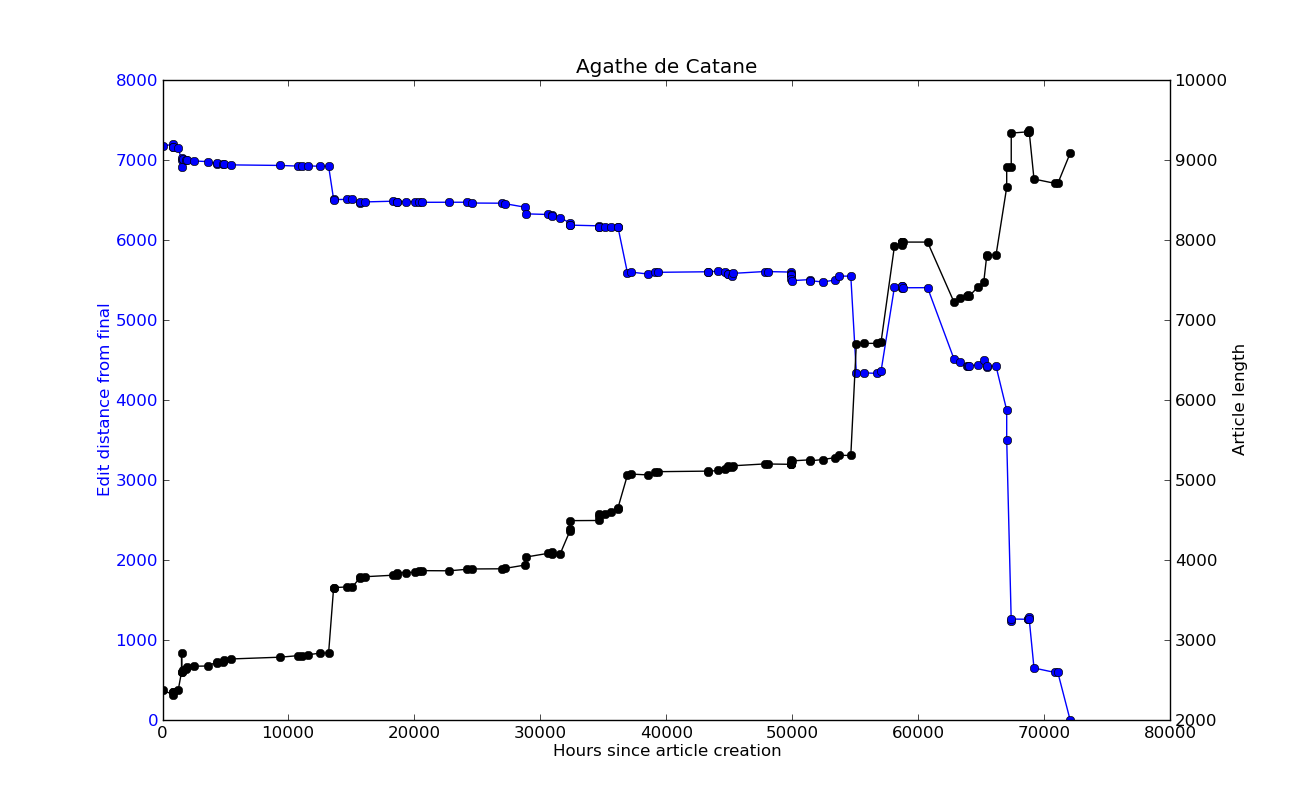
\includegraphics[width=\linewidth]{img/traj-classic/fr572796traj.png}
      \caption{\href{http://fr.wikipedia.org/wiki/index.php?curid=572796}{French
      Wikipedia, Page ID 572796 (Agatha of Catania)}}
    \end{subfigure}
  }\\
  \caption{Simple trajectory graphs.}
\end{figure}

\url{https://en.wikipedia.org/wiki/Wikipedia:Harassment#User_space_harassment}
\url{https://en.wikipedia.org/wiki/Wikipedia:Wikipedia_is_in_the_real_world}
\url{https://en.wikipedia.org/wiki/Wikipedia:Wikipedia_is_anonymous}
\url{https://en.wikipedia.org/wiki/Wikipedia:Harassment#Wikihounding}

\begin{figure}
  \begin{subfigure}[b!]{0.45\linewidth}
    \lstinputlisting[
      language=SQL,
      basicstyle=0.8\footnotesize,
      firstline=44,
      lastline=70,
    ]{discussion/sqlsnippet1.sql}
  \end{subfigure}
  \begin{subfigure}[b!]{0.45\linewidth}
    \lstinputlisting[
      language=SQL,
      basicstyle=0.8\footnotesize,
      firstline=71,
      lastline=97,
    ]{discussion/sqlsnippet1.sql}
  \end{subfigure}
  \caption{SQL snippet used to measure discrepancy between Trajectory
    calculations and distance calculations}
\end{figure}
